\documentclass[a4paper, 20pt]{article}
\usepackage[utf8]{inputenc}
\usepackage{jeffe,handout}
\usepackage{enumerate}
\usepackage{tikz}
\usetikzlibrary{arrows,shapes.gates.logic.US,shapes.gates.logic.IEC,calc}
\usepackage{hyperref}
\usepackage{aurical}
\usepackage[T1]{fontenc}

\def\lnot{\mathop{\sim}}
\def\implies{\mathop{\rightarrow}}
\def\xor{\mathop{\oplus}}

\begin{document}
\headers{CPSC 121}{ }{Winter 1, 2018}

\begin{center}
    \LARGE
    \textbf{HW 1}
    \\[1ex]
    \Large Due: 19:00, Monday, September 24, 2018  \\
\end{center}
    \LARGE
\begin{tabular}{rl}
 & \\
CS ID 1: & \rule{3cm}{0.25mm}\\
 & \\
CS ID 2: & \rule{3cm}{0.25mm}\\
 & \\
\end{tabular}
\large

\textbf{Instructions:}
\begin{enumerate}
\item Do not change the problem statements we are giving you. Simply add your solutions by editing this latex document. 
\item If you need more space, add a page between the existing pages using the \texttt{\textbackslash newpage} command.
\item Export the completed assignment as a PDF file for upload to gradescope.
\item On gradescope, upload only \textbf{one} copy per partnership. (Instructions for uploading to gradescope are posted on the assignments page of the course website.)
\end{enumerate}

\textbf{Academic Conduct:} 
I certify that my assignment follows the academic conduct rules for of CPSC 121 as outlined on the course website. As part of those rules, when collaborating with anyone outside my group, (1) I and my collaborators took no record but names away, and (2) after a suitable break, my group created the assignment I am submitting without help from anyone other than the course staff. \\
\newpage
\begin{enumerate}
\item (9 marks) One way to better understand a computational system is to look at the minimum set of primitives (simple operations) that are sufficient to express all the tasks performed by the system. In  this question, you will consider a (mythical)  ANDNOT gate, and prove that every  truth table  can be implemented  using \textbf {only}  ANDNOT gates  and the constant  \texttt  {True}. We  define  the  operation of  the  ANDNOT  gate as  follows: $x \textrm{ANDNOT} y$  is the same as  $x \land \lnot y$.
\begin{enumerate}
\item (3 marks) Show that $\lnot$ can be simulated using only ANDNOT and \texttt {True}. That is, design a logical expression that uses only ANDNOT and \texttt {True} and that, given a single proposition $p$, is logically equivalent to $\lnot p$. You must prove that your logical expression is correct using equivalence rules. (See, e.g., Epp 4ed page 35, or Dave's excellent formula sheet)

Let $\lnot x = y$ \\
$ \lnot x = y = T \land y = T \land\lnot x = T \textrm{ANDNOT} x$

% You may use tikz to draw fancy latex gates, or you can
% create them via logisim, screenshot the result, 
% upload it to this project, and then use the 
% "includegraphics" command to place it in this document.
% If you decide to use Logisim, use any of the gates available
% as the ANDNOT gate (you are not allowed to use any other
% gates, so there will be no confusion possible).
\vspace{4in}
\item (3 marks) Show that $\land$ can be simulated using only ANDNOT and \texttt {True}. That is, design a logical expression that uses only ANDNOT and \texttt {True} and that, given propositions $p$ and $q$, is logically equivalent to $p \land q$. You must prove that your logical expression is correct using equivalence rules. (See, e.g., Epp 4ed page 35, or Dave's excellent formula sheet)



\vspace{4in}
\item (3 marks)  Show that $\lor$ can be simulated using only ANDNOT and \texttt {True}. That is, design a logical expression that uses only ANDNOT and \texttt {True} and that, given propositions $p$ and $q$, is logically equivalent to $p \lor q$. You must prove that your logical expression is correct using equivalence rules. (See, e.g., Epp 4ed page 35, or Dave's excellent formula sheet)
\vspace{4in}
\end{enumerate}
Since for every truth table over $k$ atomic propositions, we can write a propositional form that matches the truth table using $\lnot$, $\land$ and $\lor$, your answers to parts~(a), (b) and~(c) show that you every propositional form is logically equivalent to a propositional form that uses only ANDNOT and \texttt {True}.

Addendum: when we use a computational system, such as a circuit built out of gates, or (later in the course) regular expressions, we like it to have as many features as possible since it makes it more convenient for us (think of how painful it would be to design circuits using only ANDNOT and \texttt {True}. Or using only NAND gates!) On the other hand, when we want to reason about what this system can or can not do, we like to use the smallest possible set of features, because it's easier to think about a small set of features than a large one (there are fewer cases to consider). That's why proving that every circuit can be designed using only ANDNOT and \texttt {True} can be useful.
\newpage
\item (8 marks) The truth table below defines the truth value of $s$ for each combination of truth values of $x_0,x_1,x_2$ and $x_3$.

\begin{tabular}{|c|c|c|c||c|}
\hline
$x_0$ & $x_1$ & $x_2$ & $x_3$ & $s$\\
\hline
\hline
F & F & F & F & T\\
\hline
F & F & F & T & F\\
\hline
F & F & T & F & T\\
\hline
F & F & T & T & T\\
\hline
F & T & F & F & F\\
\hline
F & T & F & T & T\\
\hline
F & T & T & F & F\\
\hline
F & T & T & T & F\\
\hline
T & F & F & F & T\\
\hline
T & F & F & T & F\\
\hline
T & F & T & F & T\\
\hline
T & F & T & T & T\\
\hline
T & T & F & F & T\\
\hline
T & T & F & T & F\\
\hline
T & T & T & F & T\\
\hline
T & T & T & T & T\\
\hline
\end{tabular}

\begin{enumerate}
\item Find a logic formula for $s$ that uses each variable at most twice. Then verify the correctness of your formula by drawing a truth table corresponding to this formula, including the truth values of all relevant sub-formulas. Enter your response in the table below. We have provided at least as many columns as you'll need. Be sure to fill in the column headings!

\bigbreak
$ (x_0 \lor x_1) \oplus (x_2 \lor\lnot x_3) \oplus x_0 $

\LARGE
\begin{tabular}{|c|c|c|c||c|c|c|c|c|}
\hline
$x_0$ & $x_1$ & $x_2$ & $x_3$ & $\lnot x_3$ & $x_0 \lor x_1$ & $x_2 \lor\lnot x_3$ & $(x_0 \lor x_1) $ & out & & & & & & & & \oplus (x_2 \lor\lnot x_3) & \\
\hline
\hline
F & F & F & F & T & F & & &\\
\hline
F & F & F & T & F & F & & &\\
\hline
F & F & T & F & T & F & & &\\
\hline
F & F & T & T & F & F & & &\\
\hline
F & T & F & F & T & T & & &\\
\hline
F & T & F & T & F & T & & &\\
\hline
F & T & T & F & T & T & & &\\
\hline
F & T & T & T & F & T & & &\\
\hline
T & F & F & F & T & T & & &\\
\hline
T & F & F & T & F & T & & &\\
\hline
T & F & T & F & T & T & & &\\
\hline
T & F & T & T & F & T & & &\\
\hline
T & T & F & F & T & T & & &\\
\hline
T & T & F & T & F & T & & &\\
\hline
T & T & T & F & T & T & & &\\
\hline
T & T & T & T & F & T & & &\\
\hline
\end{tabular}
\large

\item Now  create a circuit with inputs $x_0,x_1,x_2,x_3$ and whose output is the value $s$ described by the truth table. Design your circuit only using AND, OR, XOR or NOT gates. Your mark will depend on using as few  AND, OR, XOR gates as possible.  


\end{enumerate}


\newpage
\item (16 marks)  Here is  a list  of  five propositional  forms  and three  circuits. This  list
  contains four pairs of logically equivalent entries (we will say a circuit is equivalent
  to a propositional form  if the propositional form describes the  value of the circuit's
  output for all possible combinations of input values). For instance, maybe $A \equiv B$,
  $C \equiv D$, $E  \equiv F$ and $G \equiv H$). First determine  the four pairs, and then
  prove for each  pair that one element of  the pair is logically equivalent  to the other
  one.
  \begin{enumerate}[(A)]
  \item $a \land \lnot b$.
  \item $(a \xor b) \lor (b \xor c)$.
  \item $\lnot ((a \implies c) \wedge \lnot (c \implies b)$.
  \item $(a \implies (\lnot b \land c)) \land (\lnot b \implies c)$.
  \item $(\lnot a \lor \lnot b) \land (\lnot a \lor c) \land (b \lor c)$.
  \item \leavevmode\lower45pt\hbox{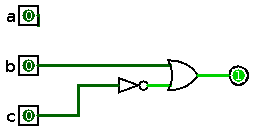
\includegraphics[scale=0.5]{ass1-q3f.png}}
  \item \leavevmode\lower45pt\hbox{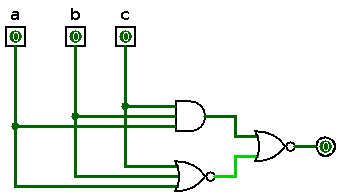
\includegraphics[scale=0.5]{ass1-q3g.png}}
  \item \leavevmode\lower45pt\hbox{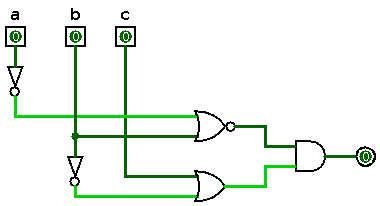
\includegraphics[scale=0.5]{ass1-q3h.png}}
  \end{enumerate}

  You are  allowed to use truth  tables to figure  out the equivalences; however  at least
  three of your proofs must use a  sequence of known logical equivalences (see Epp-4 table
  2.1.1, Epp-3  table 1.1.1, Rosen-6 table  6 in section  1.2, Rosen-7 table 6  in section
  1.3, or Dave's excellent formula sheet; you can also assume that $x \implies y \equiv \;
  {\lnot x \vee y}$ and that $x \oplus y \equiv (x \lor y)\, \land \sim\! (x \land y) \equiv
  (\lnot x \land y) \lor (x \land \lnot y)$. The fourth proof can use either a sequence of
  known logical equivalences, or a truth table.

  Hint: you might want to translate the  circuits into formulas that mirror exactly as the
  circuit is implemented, before using any logical equivalence rules.
  \newpage
\begin{enumerate}
\item \LARGE\underline{~~~~~~~~~}$\equiv$\underline{~~~~~~~~~~}\\

\begin{tabular}{rcl|l}
~~~~~~expression 1 & & expression 2~~~~~~ & reason \\
\hline
& $\equiv$ & & ~~~~~~~~~~~~~~~~~~~~~~~\\
\hline
& $\equiv$ & & ~~~~~~~~~~~~~~~~~~~~~~~\\
\hline
& $\equiv$ & & ~~~~~~~~~~~~~~~~~~~~~~~\\
\hline
& $\equiv$ & & ~~~~~~~~~~~~~~~~~~~~~~~\\
\hline
& $\equiv$ & & ~~~~~~~~~~~~~~~~~~~~~~~\\
\hline
& $\equiv$ & & ~~~~~~~~~~~~~~~~~~~~~~~\\
\hline
& $\equiv$ & & ~~~~~~~~~~~~~~~~~~~~~~~\\
\hline
& $\equiv$ & & ~~~~~~~~~~~~~~~~~~~~~~~\\
\hline
& $\equiv$ & & ~~~~~~~~~~~~~~~~~~~~~~~\\
\hline
& $\equiv$ & & ~~~~~~~~~~~~~~~~~~~~~~~\\
\hline
\end{tabular}
\large
\newpage
\item \LARGE\underline{~~~~~~~~~}$\equiv$\underline{~~~~~~~~~~}\\

\begin{tabular}{rcl|l}
~~~~~~expression 1 & & expression 2~~~~~~ & reason \\
\hline
& $\equiv$ & & ~~~~~~~~~~~~~~~~~~~~~~~\\
\hline
& $\equiv$ & & ~~~~~~~~~~~~~~~~~~~~~~~\\
\hline
& $\equiv$ & & ~~~~~~~~~~~~~~~~~~~~~~~\\
\hline
& $\equiv$ & & ~~~~~~~~~~~~~~~~~~~~~~~\\
\hline
& $\equiv$ & & ~~~~~~~~~~~~~~~~~~~~~~~\\
\hline
& $\equiv$ & & ~~~~~~~~~~~~~~~~~~~~~~~\\
\hline
& $\equiv$ & & ~~~~~~~~~~~~~~~~~~~~~~~\\
\hline
& $\equiv$ & & ~~~~~~~~~~~~~~~~~~~~~~~\\
\hline
& $\equiv$ & & ~~~~~~~~~~~~~~~~~~~~~~~\\
\hline
& $\equiv$ & & ~~~~~~~~~~~~~~~~~~~~~~~\\
\hline
& $\equiv$ & & ~~~~~~~~~~~~~~~~~~~~~~~\\
\hline
& $\equiv$ & & ~~~~~~~~~~~~~~~~~~~~~~~\\
\hline
& $\equiv$ & & ~~~~~~~~~~~~~~~~~~~~~~~\\
\hline
& $\equiv$ & & ~~~~~~~~~~~~~~~~~~~~~~~\\
\hline
& $\equiv$ & & ~~~~~~~~~~~~~~~~~~~~~~~\\
\hline
& $\equiv$ & & ~~~~~~~~~~~~~~~~~~~~~~~\\
\hline
& $\equiv$ & & ~~~~~~~~~~~~~~~~~~~~~~~\\
\hline
& $\equiv$ & & ~~~~~~~~~~~~~~~~~~~~~~~\\
\hline
& $\equiv$ & & ~~~~~~~~~~~~~~~~~~~~~~~\\
\hline
& $\equiv$ & & ~~~~~~~~~~~~~~~~~~~~~~~\\
\hline
\end{tabular}\\
\large
\newpage
\item \LARGE\underline{~~~~~~~~~}$\equiv$\underline{~~~~~~~~~~}\\

\begin{tabular}{rcl|l}
~~~~~~expression 1 & & expression 2~~~~~~ & reason \\
\hline
& $\equiv$ & & ~~~~~~~~~~~~~~~~~~~~~~~\\
\hline
& $\equiv$ & & ~~~~~~~~~~~~~~~~~~~~~~~\\
\hline
& $\equiv$ & & ~~~~~~~~~~~~~~~~~~~~~~~\\
\hline
& $\equiv$ & & ~~~~~~~~~~~~~~~~~~~~~~~\\
\hline
& $\equiv$ & & ~~~~~~~~~~~~~~~~~~~~~~~\\
\hline
& $\equiv$ & & ~~~~~~~~~~~~~~~~~~~~~~~\\
\hline
& $\equiv$ & & ~~~~~~~~~~~~~~~~~~~~~~~\\
\hline
& $\equiv$ & & ~~~~~~~~~~~~~~~~~~~~~~~\\
\hline
& $\equiv$ & & ~~~~~~~~~~~~~~~~~~~~~~~\\
\hline
& $\equiv$ & & ~~~~~~~~~~~~~~~~~~~~~~~\\
\hline
& $\equiv$ & & ~~~~~~~~~~~~~~~~~~~~~~~\\
\hline
& $\equiv$ & & ~~~~~~~~~~~~~~~~~~~~~~~\\
\hline
& $\equiv$ & & ~~~~~~~~~~~~~~~~~~~~~~~\\
\hline
& $\equiv$ & & ~~~~~~~~~~~~~~~~~~~~~~~\\
\hline
& $\equiv$ & & ~~~~~~~~~~~~~~~~~~~~~~~\\
\hline
& $\equiv$ & & ~~~~~~~~~~~~~~~~~~~~~~~\\
\hline
& $\equiv$ & & ~~~~~~~~~~~~~~~~~~~~~~~\\
\hline
& $\equiv$ & & ~~~~~~~~~~~~~~~~~~~~~~~\\
\hline
& $\equiv$ & & ~~~~~~~~~~~~~~~~~~~~~~~\\
\hline
& $\equiv$ & & ~~~~~~~~~~~~~~~~~~~~~~~\\
\hline
\end{tabular}
\large
\newpage
\item \LARGE\underline{~~~~~~~~~}$\equiv$\underline{~~~~~~~~~~}\\
\newpage
\end{enumerate}
\newpage
\item  Design  a circuit that  takes five inputs $x_1$,  $x_2$, $x_3$, $x_4$,  $x_5$ and
  outputs \texttt  {true} if (and only  if) there is an ``isolated value''. We say an input is {\em isolated}
  if it is T and in-between two F values, or F and in-between two T values. 
 For instance, your  circuit should output  \texttt {true} in  the following
  three cases:
  \begin{itemize}
  \item  $x_1   =  \texttt{true}$,   $x_2  =   \texttt{true}$,  $x_3   =  \texttt{true}$,
    $x_4 = \texttt{false}$, $x_5 = \texttt{true}$.
  \item  $x_1   =  \texttt{false}$,  $x_2   =  \texttt{true}$,  $x_3   =  \texttt{false}$,
    $x_4 = \texttt{true}$, $x_5 = \texttt{false}$.
  \item  $x_1   =  \texttt{true}$,  $x_2   =  \texttt{false}$,  $x_3   =  \texttt{true}$,
    $x_4 = \texttt{false}$, $x_5 = \texttt{true}$.
  \end{itemize}
  but it should output \texttt {false} in these cases:
  \begin{itemize}
  \item  $x_1   =  \texttt{false}$,   $x_2  =   \texttt{true}$,  $x_3   =  \texttt{true}$,
    $x_4 = \texttt{false}$, $x_5 = \texttt{false}$.
  \item  $x_1   =  \texttt{true}$,   $x_2  =   \texttt{true}$,  $x_3   =  \texttt{false}$,
    $x_4 = \texttt{false}$, $x_5 = \texttt{true}$.
  \item   $x_1  =   \texttt{false}$,  $x_2   =  \texttt{true}$,   $x_3  =   \texttt{true}$,
    $x_4 = \texttt{true}$, $x_5 = \texttt{false}$.
  \end{itemize}
  Points given  for this question will  depend in part  on the elegance of  your solution.
  Using a truth  table will work, but will  give a very large circuit. Try  to think about
  the kinds of inputs that are (or are not) permissible instead. Justify your answer!
    \newpage
\newpage
\item Suppose you have embarked on a journey of discovery into a land occupied by sword wielders, villains, and worms. Sword wielders always tell the truth, villains always lie, and worms flip a coin to decide whether they tell the truth or lie, every time they speak. One day, your path is blocked by three fair beasts named Asuna, Sinon, and Winry Rockbell, who will only allow you to pass if you can solve their riddle, which is posted on a nearby sign. The sign reads, ``Here stands a sword wielder, a villain, and a worm. Name each and you may proceed!'' The fair beasts, in turn, say the following:
\begin{itemize}
 \item Asuna: {\Fontlukas I am a sword wielder!}
 \item Sinon: {\Fontlukas Asuna is telling the truth.}
 \item Winry Rockbell: {\Fontlukas I am a worm.}
 \end{itemize}
 Who is the sword wielder, who is the villain, and who is the worm? Prove that your choices are correct by arguing that each of the other options leads to an impossibility.
\end{enumerate}
\end{document}
